\chapter{Background}
\label{Background}

\section{Deep Learning}
In last few years, Deep Learning has been the state of the art approach for solving most computer vision problems. All related work to this project that has been carried out in recent years, are based on Deep Learning. Also, based on the promising results of this approach, it was chosen as the main method for this project. Therefore, before discussing any related work, it is best to have a brief introduction to Deep Learning. 

\subsection{Overview} \label{sec:bgoverview}
Deep Learning is a sub-field of machine learning concerned with Artificial Neural Networks (ANNs) with more than a few layers. ANNs are computing systems inspired by biological neural networks in the brain. ANNs, like brain, are based on collection of connected units called artificial neurons. Typically, these neurons are organised in layers. Figure \ref{fig:ANN} demonstrates the architecture of a simple ANN.

\begin{figure}
    \centering
    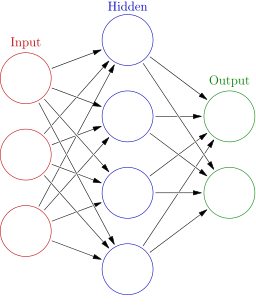
\includegraphics[scale=0.4]{ANN}
    \caption{A simple Artificial Neural Network (ANN) \caplicense{By \url{Glosser.ca} [CC BY-SA 3.0], via Wikimedia Commons}}
    \label{fig:ANN}
\end{figure}

Data is fed to the network by input neurons in form of numerical vectors. Input neurons are connected to other neurons in the network and pass the data through these connections. Each connection has a weight associated with it. Any vector of data that passes through a connection is multiplied by the weight of that connection. At each neuron, a function (e.g. hyperbolic tangent) is applied to all the input vectors that reach the neuron through different connections, and the result is passed to the other connected neurons. Data flows though the network by input neurons; each layer of neurons performs some kind of transformation on it, and the end result becomes available at output neurons.

The ANN in figure \ref{fig:ANN} is a very simple network with just three layers. Deep neural networks usually consist of many more layers with different types of neurons. For example GoogLeNet \cite{googlenet}, which was the winner of The ImageNet Large Scale Visual Recognition Challenge (ILSVRC) 2014, is a 22 layer neural network with 7 different types of layers. Some of the current state of the art deep neural networks have more than a hundred layers. 

\begin{figure}
    \centering
    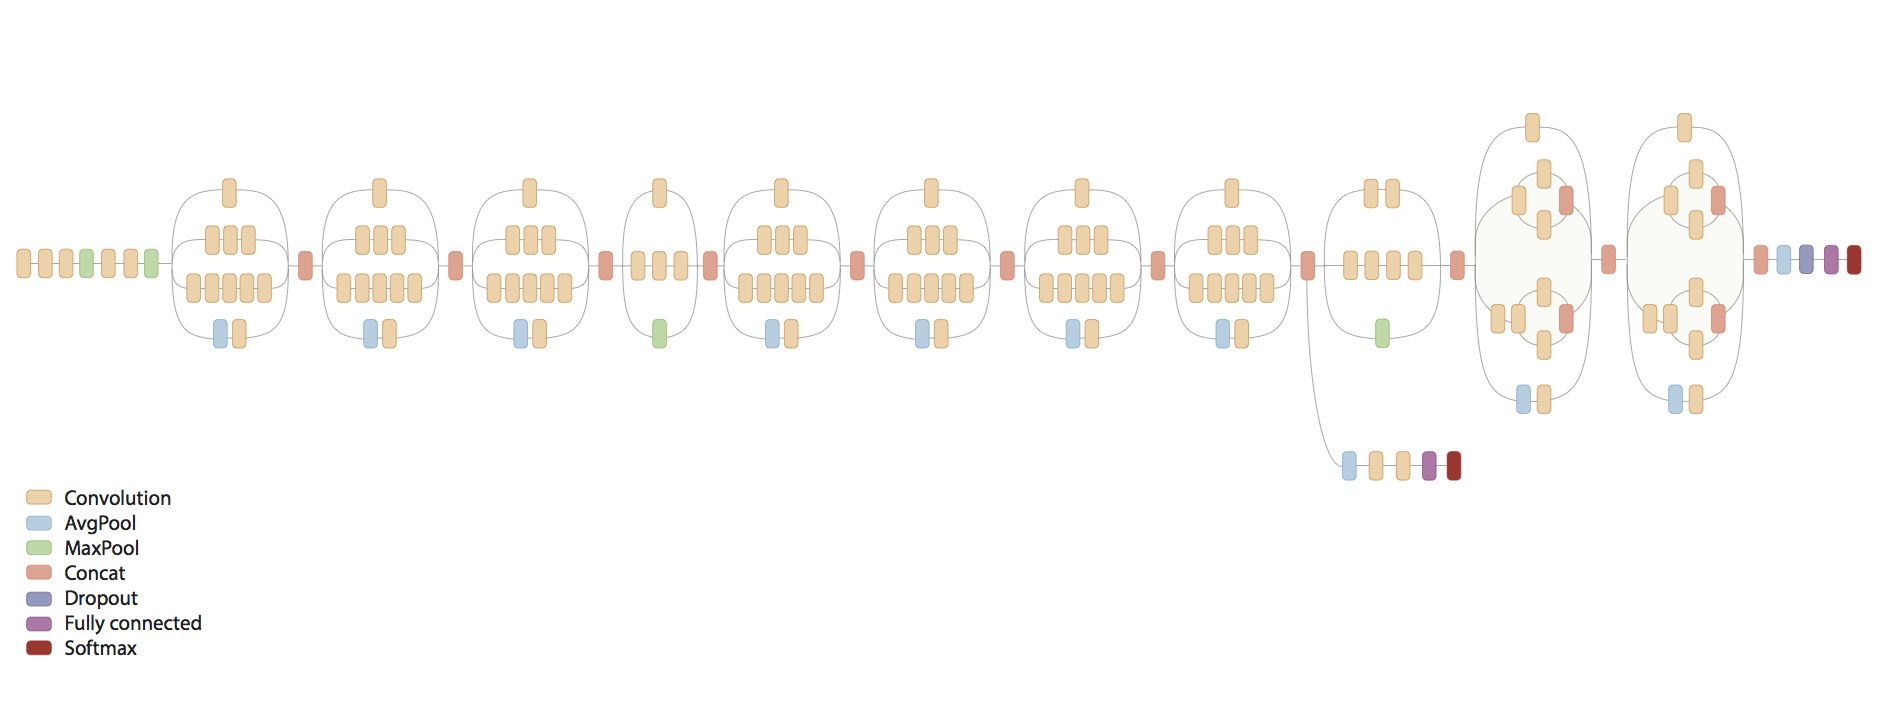
\includegraphics[width=\textwidth]{googlenet}
    \caption{GoogLeNet \cite{googlenet}, a deep neural network \caplicense{Picture courtesy of \url{https://github.com/tensorflow/models/tree/master/inception}}}
    \label{fig:googlenet}
\end{figure}

Two main applications of deep neural networks are in classification and regression problems. In classification problems, the aim is to predict the correct category for each input sample from a set of predefined classes. For example, predicting the specie of animals by looking at their pictures. On the other hand, in regression problems, the goal is to estimate the relationship between variables. For example, estimating the age of people (dependent variable) by looking at a photo of their face (facial structure as independent variable); Or in case of this project, the pixel-wise surface normals based on the RGB image of a scene. 

To achieve these goals, a suitable network architecture (based on the problem) should be selected and the optimal weights for its connections have to be determined. Network architecture is usually chosen based on the architectures that are used in similar problems and the prior experience of the expert.  But it is not possible to manually determine the optimal weights of a network; because deep neural networks usually have millions of parameters (e.g. 61 million for AlexNet \cite{alexnet} and 138 million for VGG-16 \cite{vgg} architecture) \cite{dnnparameters}. In practice, usually these parameters are initialised by random numbers and the optimal value of them is learned in a process called training. In next sections, the overall network architecture, building-blocks of the deep neural networks which are relevant to this project, and the training process are introduced.  

\subsection{Architecture}

In last few years, Convolutional Neural Networks (CNNs) have been the most popular type of deep neural networks in field of computer vision \cite{cnnpopular}. In this chapter, we focus on this type of deep neural networks. 

CNNs usually consist of three different types of layers: Convolutional, Pooling and Fully Connected. Figure \ref{fig:cnn} demonstrates an example of such networks. It is worth noting that popular CNN architectures differ in the number, arrangement, and the connection between these layers. In following sections, these layers are discussed in more details.

\begin{figure}
    \centering
    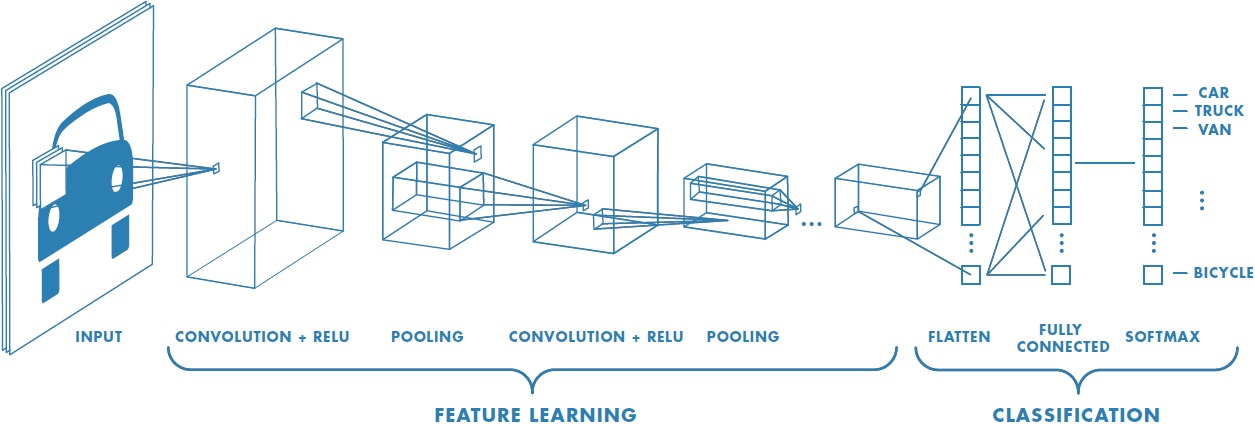
\includegraphics[width=\textwidth]{CNN}
    \caption{Example of a CNN architecture for image classification \caplicense{Diagram courtesy of The MathWorks, Inc. \url{https://uk.mathworks.com/discovery/convolutional-neural-network.html}}}
    \label{fig:cnn}
\end{figure}

\subsubsection{Convolutional Layer}

Convolutional layers are used to extract features from data. In case of images, these features can range from low level details such as edges to very abstract concepts such as human face. Convolutional layers work based on convolution operation. In each layer, a set of features in form of convolution kernels (also called filters) are applied over the input. The output of these operations is called feature map and specifies the regions in the input that the corresponding feature is present. By stacking convolutional layers in a network, input data is represented in form of feature maps in different levels of abstraction.    

\begin{figure}[h]
    \centering
    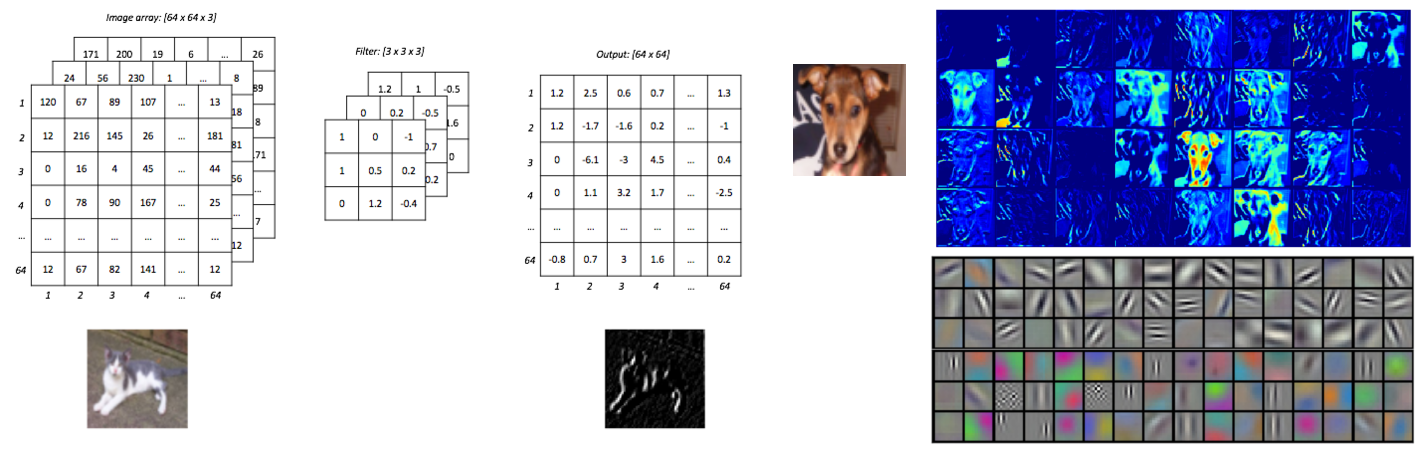
\includegraphics[width=\textwidth]{CNNFilters}
    \caption{Left: Applying a filter (convolution kernel) on input image and the resulting feature map. Right top: Heat-map visualisation of feature maps corresponding to 32 different filters. \\ Right bottom: Visualisation of 96 filters of first convolution layer in AlexNet \cite{alexnet} \caplicense{Left and Right top images are courtesy of \url{http://www.subsubroutine.com/sub-subroutine/2016/9/30/cats-and-dogs-and-convolutional-neural-networks}}}
    \label{fig:CNNFilters}
\end{figure}

In traditional methods of computer vision, the filters for feature extraction were used to be designed by the experts. The main advantage of CNNs is in their ability to automatically learn the suitable filters for each problem in the training process. By learning the best features to represent the data, CNNs get much better results in classification and regression analysis of data in comparison to traditional methods. 

To design the architecture of a CNN, for each convolutional layer, value of several parameters are needed to be decided: the number of filters in a layer, the size (height and width) of these filters, strides, and padding. To apply a filter on input matrix, the filter window shifts over the input data; computing a value for each position in the feature map. Strides parameter specifies how many pixels the filter window should move in each dimension over the input to compute a value in the feature map. For example, a stride of (2,2) moves the filter windows two pixels in each dimension, resulting in a smaller feature map than the input. Even with a stride of (1,1), the size of feature map shrinks. To keep the feature map the same size as input, a zero-padding can be applied on input data. 

\begin{figure}
    \centering
    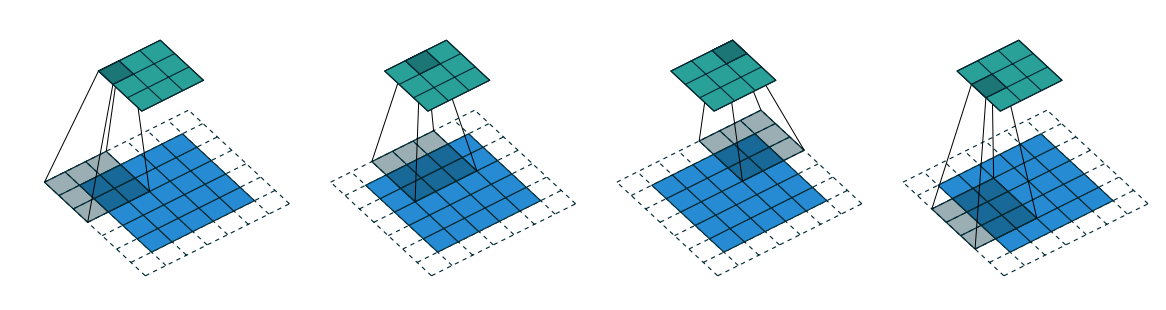
\includegraphics[width=\textwidth]{StridePadding}
    \caption{Convolution on an input with 5x5 size (Blue), by a kernel size of 3x3 (Gray), in 2x2 strides with zero padding; resulting in a 3x3 feature map (Green) \cite{stridepadding}.}
    \label{fig:stridepadding}
\end{figure}

\subsubsection{Activation Layer}
It is convention to apply a nonlinear activation layer after each convolutional layer. The main purpose of this layer is to add non-linearity to the network. The activation layer applies a function to all the values of input data from last layer. The most common activation function in CNNs, is the Rectifier: \(f(x) = max(0, x)\). In network architecture diagrams, usually the activation layer following a convolutional layer is not depicted.  

\subsubsection{Pooling Layer} \label{sec:pooling}

Usually after some convolutional layers in a CNN, a pooling layer is applied. There are several different types of pooling layers such as max pooling, average pooling, and L2-Norm pooling. In this layer a filter (usually of size 2x2) is applied to the input with strides of same length (2x2). In contrast to convolutional layers that compute the weighted sum over the region covered by the filter, the pooling layers compute the max, average or L2-Norm of that region. Pooling (also referred to as down-sampling) layers play two important roles in a network. First, it reduces the size of the data in the network; thus lessening the computational cost. Second, because it preserves the relative position of features in the feature maps but not the exact locations, the network learns to be more general and robust to noise. 

\subsubsection{Fully Connected Layer}

The collection of convolutional, activation, and pooling layers, provides a representation of input data based on the learnt features. Another type of layers is needed to actually perform the classification or regression analysis based on the represented data. The fully connected layers provide a universal function that can learn (by adjusting the weights of their connections) to estimate the relation between variables or predict the class of the input data. Figure \ref{fig:MLP} demonstrates such layers. The fully connected layers work in the same way as traditional neural networks (as described in page \pageref{sec:bgoverview}). It is common to apply the fully connected layers at the end of the CNNs to produce the output of the network. To connect the other layers to the fully connected ones, the multi-dimensional output of those layers is first flattened into a 1D vector, then it is passed to the all input neurons of the fully connected layers (figure \ref{fig:cnn}). 

\begin{figure}
    \centering
    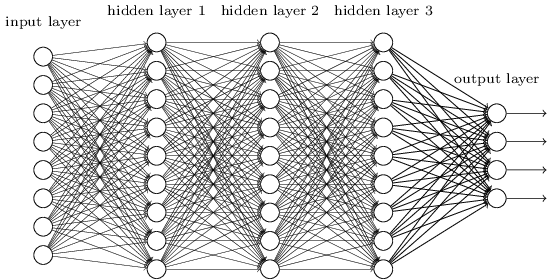
\includegraphics[scale=0.5]{MLP}
    \caption{Example of fully connected layers of a CNN \caplicense{Picture courtesy of \url{http://neuralnetworksanddeeplearning.com/chap6.html}}}
    \label{fig:MLP}
\end{figure}

In classification problems, each output neuron of the fully connected layers estimates the probability of belonging to a specific class (e.g. cat, dog, and so on.). In regression problems, each output neuron estimates the value of a dependent variable. For example in case of this project, the x, y, or z component of a normal vector, corresponding to a specific pixel in the input image. 

\subsection{Training}

In CNNs, usually the filters of the convolutional layers and the weights of the fully connected layers are initialised with random numbers. But, to produce a meaningful output, these parameters needs to be adjusted based on the problem. Training is a process in supervised learning to determine the near-optimal values of these parameters. In supervised learning, pairs of input samples and the corresponding desired outputs for a problem are needed. For example, in the problem of age estimation based on the face photo, the pairs of photos of different people and their ages are needed. Based on these (input,desired output) samples, an optimiser can calculate the appropriate values for the parameters of a network. After training, by having a network that its parameters are customised to the problem, it is possible to estimate the output for input samples that are new to the network. 

To train a neural network, in addition to an optimiser, a cost function is also needed. A cost function is any function that accepts the computed output of the network and the desired output as arguments, and returns a cost value that is an indicator of error between these values. 

Training a network is performed in iterations. In each step, a sample (or a small batch of samples) is chosen from the data set. First, this input is passed to the network and the predicted output of the network is computed. Then, the predicted output and the desired output in the data set is passed to the cost function and the cost value is computed. Finally, the optimiser calculates the adjustments to the parameters of the network based on the cost value. Most of the common optimisers, calculate these adjustments based on the gradient of cost function in respect to all parameters of the network. After each iteration, the parameters of the network are updated. 

Usually, to have an idea of the accuracy of a network, the data set is divided into two separate data sets: training and testing. The network is trained on the training data set; then, its estimated output for the samples of the testing data set is computed. The difference between these values and the desired outputs of the testing data set is an indicator of how good the network is expected to perform for samples out of the training data set.

In the past, the most frequently used optimiser for training the deep neural networks was the Stochastic Gradient Descent (SGD). This optimiser approximates the gradient at each sample (or small batch), then updates the parameters of the network based on this value multiplied by a learning rate. The learning rate is a number usually close but less than one, that determines how fast the parameters of the network should change in training process. Having a single learning rate for all the parameters of the network (while different parameters need different rates) that is fixed during training is one of the main disadvantages of this optimiser. 

In this project the Adam optimiser \cite{adam} is used for training the network. The Adam optimiser, maintains a learning rate for each network parameter which separately adapts as learning unfolds. Based on the findings of a recent survey \cite{bestoptimiser}, Adam is currently the best optimiser for use in projects such as this one. 

Likewise, there are many different choices available for the cost function. Some of the most common ones are Mean Squared Error, Mean Absolute Error, and Categorical Cross Entropy. Besides popular cost functions, it is also common to use a custom cost function for a problem.  

Finally, the last term relevant to training process that is worth noting is the epoch. An epoch consists of one complete training cycle on the samples in the data set. Normally, more than one epoch is needed to train a network. 

\subsection{Transfer Learning}

As mentioned earlier, normally the parameters of a network is initialised by random values. In order to learn the best parameters for the network, a lot of time and a large data set for training is needed. As network architecture gets more sophisticated, the need for larger data sets and more training time increases. Therefore, if the training time or the size of the data set is a constraint, getting acceptable results is less likely. An effective method to solve this problem is the use of the transfer learning. In transfer learning, a pre-trained network (or a part of it) is fine-tuned for use in current problem. For example the lower layers of an image classification network such as VGG-16 \cite{vgg}, can be used for feature extraction in a regression problem. 

By initialising the parameters of the network to compatible parameters of another network that is trained on a larger data set and in a relevant problem, it is more likely that the optimal parameters of the network are close to the initial values; thus potentially, less number of training iterations is needed for achieving acceptable outputs.

\subsection{Data Augmentation}

Another technique to compensate for the small training data set is data augmentation. Some data transformations on the data set samples can make considerable changes in the inputs while preserving the desired outputs. For example, moderate changes in contrast or saturation of an image of a dog does not affect the specie of the animal (i.e. the desired output). But, these changes produce different training samples for the network. By using carefully selected data augmentations, the size of a data set increases considerably. Another positive side effect of using data augmentation is decreasing the chance of over-fitting. An over-fitted network losses its generality and robustness to noise.   

\section{Related Work} \label{sec:relatedwork}

Before discussing the related work on surface normal estimation from RGB images, it is best to mention a similar problem: estimating the depth map from RGB images. By having the depth map of a scene, it is possible to calculate the pixel-wise surface normals by simply fitting a least-square plane for the neighbouring sets of points in the 3D point cloud (discussed in section \ref{sec:surfnormmap}). However, depth map estimation is also a challenging task. In fact, some of the works discussed in this section \cite{eigen,dharmasiri}, attempt to jointly estimate depth and surface normal maps. Independent methods for depth map estimation have been proposed, too; methods such as Markov Random Fields \cite{saxena}, focus information and higher order statistics \cite{jaeseung}, semantic labels \cite{liusemantic}, deep convolutional neural fields \cite{liucnf}, and multi-scale deep neural networks \cite{eigendepth}.     

In recent years, there have been several attempts to tackle the problem of surface normal estimation from RGB images. In this section, some of the better performing works are discussed; interestingly, all of them are based on convolutional neural networks. Although all of these methods use CNNs, the main difference between them lies in their network architecture. They all use the same data sets and metrics for training and evaluation (which are addressed in chapter \ref{Dataset} and chapter \ref{ExperimentsAndResults}, respectively). Therefore, the main focus of this section in discussing these methods, is the architecture of underlying CNN models.

\citeauthor*{wang} \cite{wang} propose a network architecture that consists of three sub-networks: a top-down network, a bottom-up network, and a fusion network  (figure \ref{fig:wang}). The top-down network takes the RGB image as input and predicts two complementary global interpretations of the scene: a coarse estimation of the surface orientations, and the cuboidal layout of the room. For the bottom-up network, a sliding window on the input image, extracts patches of the image. The bottom-up network takes these patches one after another to generate two types of local image interpretations for the whole image: estimated pixel-wise surface normals, and semantic edge labels (convex, concave, and occlusion). 

They also calculate the vanishing points of the input image (based on the non-neural network approach of \citeauthor*{vanishingpoints} \cite{vanishingpoints}) and compute the vanishing point-aligned coarse interpretation of the scene, based on the output of the top-down network. The concatenation of the four outputs of the other sub-networks with the input image and the vanishing point-aligned coarse output, is used as the input to the fusion network. At last, the fusion network estimates the final pixel-wise surface normals, by using a sliding window on the input image and based on the interpretations provided by other sub-networks.

\begin{figure}[h]
    \centering
    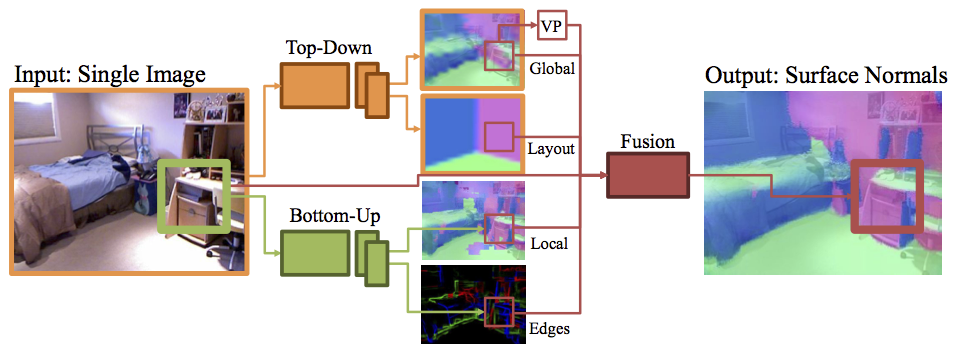
\includegraphics[width=0.85\textwidth]{Wang}
    \caption{An overview of the network architecture designed by \citeauthor*{wang} \cite{wang}}
    \label{fig:wang}
\end{figure}

Because of the computational costs and difficulty in training a network that globally estimates the pixel-wise surface normals, \citeauthor*{wang} use a sliding window to estimate the local surface normals. But, only by looking at local patches of the image, it is difficult to get the results that are consistent within the whole picture. By using a fusion network that considers the coarse global interpretation of the scene, while looking at local patches, they manage to produce 31\% better results in comparison to output of the bottom-up network (increase from 27.2\% to 39.5\% within \ang{11.25} of error).  

Moreover, they argue that the design of deep neural networks can benefit greatly by incorporating the insights from past research in 3D scene understanding; notably, knowledge about the room layout and edge labels. 

Despite the fact that by adding all the additional interpretations (i.e., room layout, edge labels, and vanishing point-aligned coarse output) to the fusion network, the percentage of the normal vectors within \ang{11.25} error improves by 11.9\% (from 39.5\% to 44.2\%), just adding the vanishing point-aligned coarse output results in 8.1\% better outputs (from 39.5\% to 42.7\%). 

Therefore, contrary to the opinion of \citeauthor*{wang}, the small benefits gained by using room layout and edge label interpretations, might not worth the additional complexity that they impose on the network. Furthermore, as recent achievements by convolutional neural networks have shown, focusing on exploiting the feature extraction capabilities of CNNs may be a better choice than using hand-crafted features like room layout or edge labels.     

\citeauthor*{eigen} \cite{eigen} also estimate the coarse global output and the local surface orientations, but instead of independently computing these outputs and combining them by a separate fusion network, they design a multi-scale deep network (figure \ref{fig:eigen}). 

\begin{figure}[h]
    \centering
    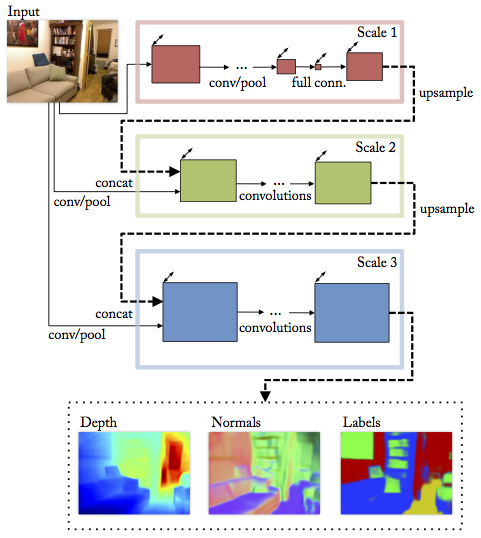
\includegraphics[scale=0.57]{Eigen}
    \caption{An overview of the network architecture designed by \citeauthor*{eigen} \cite{eigen}}
    \label{fig:eigen}
\end{figure}

In their model, first, the input image (of size 320x240) is fed to the Scale 1 network which predicts a coarse global output based on the entire image area. However, instead of directly estimating the coarse surface orientations, this network reshapes the output of the fully connected layers to 64 feature maps of size 19x14. These feature maps are up-sampled by a factor of 4 (i.e., 74x55), and the result is passed to the Scale 2 network. 

To produce predictions at a mid-level resolution, a single layer of convolution and pooling with finer strides is applied to the input image and the resulted feature maps are concatenated with the up-sampled feature maps of Scale 1 and are passed to the Scale 2 network. The output of the second scale is a 74x55 prediction of surface orientations which gets up-sampled to size of 147x109. 

Finally, by concatenating the up-sampled output of Scale 2 with the feature maps generated by a single layer of convolution and pooling at yet finer stride, the Scale 3 network predicts the surface orientations in more detail (at half resolution of the original image). 

Normally in CNNs, the size of the filters in convolutional/pooling layers is relatively small (less than 10x10) in comparison to the input data. Therefore, these layers are suited to extract the local features of the data. In contrast, fully connected layers in a CNN have connections to all the feature maps of the last convolutional/pooling layer of the network. As a result, the fully connected layers have a global view of the input data. 

In the network architecture of \citeauthor*{eigen}, the main difference between the Scale 1 and the other scales of the network is in existence of fully connected layers in Scale 1. These layers provide a global view of the scene and enable the Scale 1 network to estimate the coarse global feature maps. The other scales, by using the output of Scale 1 along the feature maps generated from the input image, are able to refine the local details in consistence with the whole scene. It worth noting that the Scale 2 and Scale 3 networks, estimate the pixel-wise normal vectors (x,y,z components), by using 3 filters in their last convolutional layers. 

In comparison to work of \citeauthor*{eigen}, \citeauthor*{wang} use fully connected layers in all of their sub-networks. The local view of their bottom-up and fusion networks, is a result of using a sliding window at the input of these networks. By doing so they can process the input data in higher detail, while keeping the computational costs manageable. In the model of \citeauthor*{eigen}, the resolution of input image to different scales is determined by the length of strides in the first single convolutional/pooling layers in each scale. 

For the Scale 1 network of \citeauthor*{eigen}, they try both of AlexNet \cite{alexnet} and VGG-16 \cite{vgg} network architectures. They initialise the parameters of these networks with parameters of respective models that are trained on ImageNet data set \cite{imagenet}. 

In training phase, because of the computational costs, first they jointly train both Scale 1 and 2 networks; then, they fix the parameters of these scales and train the Scale 3 network. They show that the more sophisticated model (VGG-16) achieves 13.3\% better result (from 39.2\% to 44.4\% within \ang{11.25} error) in comparison to the other one. 

\pagebreak

\citeauthor*{dharmasiri} \cite{dharmasiri} design a network architecture that is fundamentally very similar to work of \citeauthor*{eigen}. They extend the model of \citeauthor*{eigen}, by adding parallel layers in Scale 2 and 3 of the original network (figure \ref{fig:dharmasiri}). These parallel layers are adapted to estimate the pixel-wise depth and surface curvature, based on the input image. The network is configured to jointly estimate the depth, surface normals, and surface curvature. 

\begin{wrapfigure}{r}{0.45\textwidth}
    \centering
    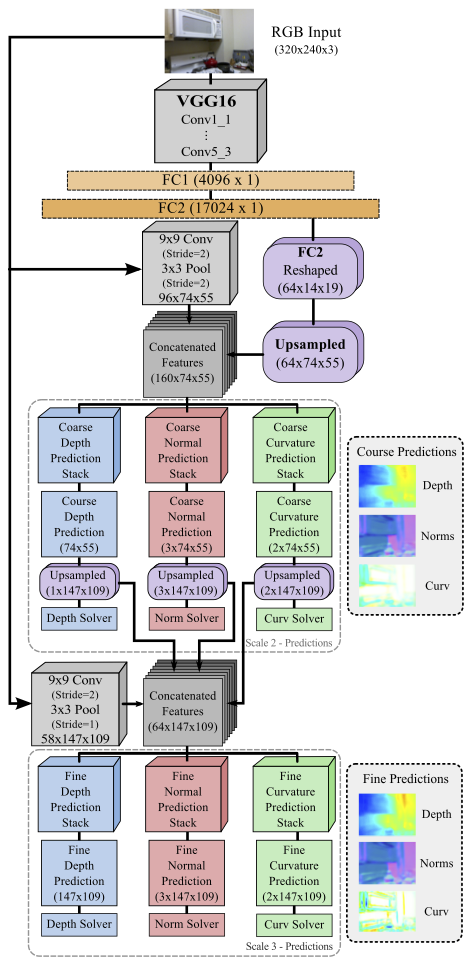
\includegraphics[width=\linewidth]{Dharmasiri}
    \caption{An overview of the network architecture designed by \citeauthor*{dharmasiri} \cite{dharmasiri}}
    \label{fig:dharmasiri}
\end{wrapfigure}

They argue that by using multi-task learning, each task benefits from having access to the data representation provided by other similar tasks. For example, the normal estimation layers in Scale 3, receive the concatenated outputs of all the layers in Scale 2; thus, theoretically they have access to more extracted features about the input image. This idea is similar to work of \citeauthor*{wang} in terms of combining different types of extracted features to enhance the performance of the network. Likewise, the enhancements gained by adding these additional representations to the network (from 43.6\% to 44.9\% within \ang{11.25} error), may not worth the complexity that they introduce to the network.      

Finally, \citeauthor*{bansal} \cite{bansal} propose a novel network architecture, based on hypercolumn representation, that achieves state of the art results in task of surface normal estimation. 

In conventional CNNs, the fully connected layers receive their input only from the last convolutional/pooling layer of the network, which extracts the features with highest level of abstraction. This high level feature representation of input data is exactly what is needed for classification tasks such as classifying the furniture in a room ; after all, the overall shape of an object is a more relevant factor than low level details such as pose or illumination. But in finer grade tasks such as normal estimation, these low level details are exactly what matters most. Therefore, in such applications, the last convolutional/pooling layer is not the optimal representation. 

Based on this reasoning, \citeauthor*{hariharan} \cite{hariharan} introduce hypercolumn representation in CNNs. They define the hypercolumn at a pixel as a feature vector formed by concatenating the convolutional responses of a CNN, corresponding to the location of that pixel. In other words, in each feature map in a convolutional layer, the value corresponding to the location of the input pixel is identified. All these values across the layers of the network, are concatenated to form a hypercolumn feature vector. In contrast to the feature maps of the last convolutional/pooling layer, a hypercolumn feature vector can capture coarse, mid, and fine-level details. 

\citeauthor*{bansal} \cite{bansal} use the convolutional/pooling layers of VGG-16 \cite{vgg} architecture (figure \ref{fig:vgg}) in their network. On top of VGG-16 layers, two additional convolutional layers are applied. The hypercolumn features are extracted from the \( 1_2,2_2,3_3,4_3,5_3\) layers of the VGG-16 model along with the last additional convolutional layer. The fully connected layers accept the hypercolumn feature vector of a pixel as input, and predict the surface normal vector for that pixel (figure \ref{fig:bansal}).    

\begin{figure}[h]
    \centering
    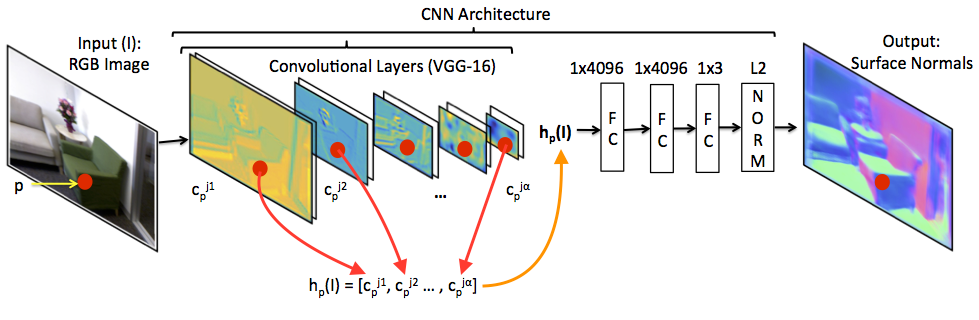
\includegraphics[width=\textwidth]{Bansal}
    \caption{An overview of the network architecture designed by \citeauthor*{bansal} \cite{bansal}}
    \label{fig:bansal}
\end{figure}

In training, instead of using all the pixels of an image, 1000 pixels per image are randomly sampled and the cost function calculates the error between the predicted and the desired normal vectors for these pixels. By doing so, the memory usage remains in bound and also the chance of over-fitting is reduced. 

Although at first glance, it may look that by randomly sampling the pixels, the spatial information is lost, but in practice the hypercolumn vectors contain high level features from the upper layers of the network. 

In fact, they show that the features of the hypercolumn vector should be selected from a combination of low, mid, and high parts of the network; otherwise, the performance of the network suffers considerably. For example, using only low and mid parts of the network (\(1_1,1_2,3_3\) layers) degrades the performance by 45\% (from 42.0\% to 23.1\% within \ang{11.25} error) in comparison to using low, mid, and high parts (\(1_2,3_3,5_3\) layers).

\begin{figure}[h]
    \centering
    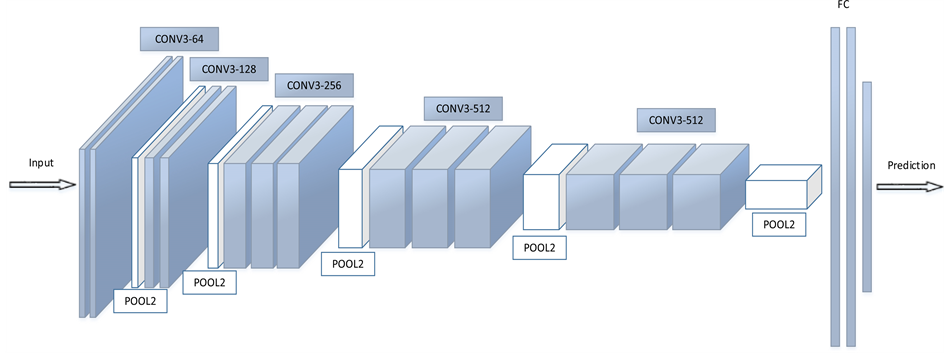
\includegraphics[width=\textwidth]{VGG}
    \caption{An overview of the VGG-16 \cite{vgg} network architecture. \caplicense{Diagram courtesy of \citeauthor*{vggdiagram} \cite{vggdiagram}}}
    \label{fig:vgg}
\end{figure}

To summarise, recent work in surface normal estimation from RGB images can roughly categorised into two groups. On the one hand, \citeauthor*{wang} \cite{wang} and \citeauthor*{dharmasiri} \cite{dharmasiri} combine features extracted by task-specific sub-networks (room layout, edge labels, depth, curvature and so on) to enrich and diversify the data representations. Although these sub-networks add complexity and computational costs to the system, their results are only a few percent better than the simpler networks. On the other hand, \citeauthor*{eigen} \cite{eigen} and \citeauthor*{bansal} \cite{bansal} solely use the features that are learnt by the network layers. While in network architecture of \citeauthor*{eigen}\cite{eigen}, the focus is on the features that are learnt at the last layer of each of the three scales, in work of \citeauthor*{bansal} the features are extracted from six different layers. On the whole, considering the relative simplicity and better results of these architectures, leaving the task of feature extraction to the CNNs and avoiding the use of task-specific representations looks as a better choice. Also, based on the findings of \citeauthor*{bansal}\cite{bansal}, using more representations at various levels of abstraction, may have a positive effect on the final results. 